\documentclass{article}
\usepackage{graphicx}
\title{Homework 5}
\author{Brandon Kujawa}
\begin{document}
\maketitle

\section*{Question 2.}
The cron script that I have created will run every 1 minute and will run the bash script that I have created. The bash script checks if the a file to see how many commits have been made. If it is less than 10 it makes a new commit.
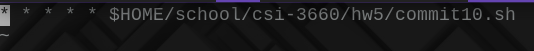
\includegraphics[scale=.45]{crontab.png} \\
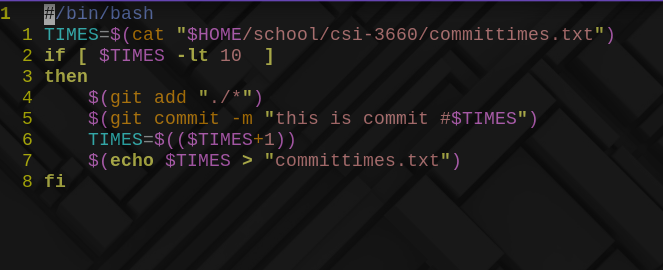
\includegraphics[scale=.45]{commitscript.png}

\section*{Question 3.}
\subsection*{a.}
The bash script that is written for this question will check if a file code.txt is created. If is is not it will create it, create a git project, make a commit then push the project to my github account.
\subsection*{b.}
In this section the bash script will use the diff command to check if any files have changed since the last time the command has ran if they have this script will add them to a commit and push the changes.

\end{document}

